\documentclass[12pt]{article}
\usepackage{epsf,epic,eepic,eepicemu}
\usepackage{amsmath, amsthm}
%\documentstyle[epsf,epic,eepic,eepicemu]{article}
\usepackage[utf8]{inputenc}
\usepackage[IL2]{fontenc}
\usepackage[czech]{babel}
\usepackage{pbox}
\usepackage{url}
\usepackage{graphicx}
\usepackage[margin=1cm]{caption}


\newtheorem{tvrz}{Tvrzení}
\theoremstyle{definition}
\newtheorem{definice}{Definice}

\begin{document}
%\oddsidemargin=-5mm \evensidemargin=-5mm \marginparwidth=.08in
%\marginparsep=.01in \marginparpush=5pt \topmargin=-15mm
%\headheight=12pt \headsep=25pt \footheight=12pt \footskip=30pt
%\textheight=25cm \textwidth=17cm \columnsep=2mm \columnseprule=1pt
%\parindent=15pt\parskip=2pt

\begin{center}
\bf Semestralní projekt MI-PAR 2015/2016:\\[5mm]
    Paralelní algoritmus pro hledání minimálního Steinerova stromu	\\[5mm]
       Libor Vytlačil\\
       Vladimír Mlázovský\\[2mm]
magisterské studijum, FIT ČVUT, Kolejní 550/2, 160 00 Praha 6\\[2mm]
\today

\vspace{2cm}

\includegraphics[width=0.3\textwidth]{obr/tree.png}
\end{center}
\newpage
\tableofcontents
\newpage
\section{Definice problému a popis sekvenčního algoritmu}
\subsection{Formulace řešeného problému}
Nejprve zformulujeme problém, který naše úloha řeší, a vysvětlíme potřebné pojmy.

Pro zadaný graf\footnote{Předpokládá se souvislý neorientovaný neohodnocený konečný graf bez smyček. Tento předpoklad platí pro každý výskyt pojmu graf v této práci, není-li explicitně řečeno jinak.} $G=(V,E)$
a množinu $\emptyset\neq A\subseteq V(G)$ nalezněte minimální\footnote{z hlediska počtu uzlů} Steinerův strom $T_A$.

Steinerův strom je klíčovým pojmem zadání. Uveďme proto jeho definici.
\begin{definice}
	Buď $G=(V,E)$ graf a $\emptyset\neq A\subseteq V(G)$. Steinerův strom v grafu $G$ pro množinu $A$ je podstrom grafu $G$, který obsahuje všechny uzly z množiny $A$. Značíme ho jako $T_A^G$ a nebo jen $T_A$, pokud je z kontextu jasné, o jakém grafu $G$ se hovoří. Množině $A$ někdy říkáme terminální množina.
\end{definice}
Naše řešení pracuje s pojmem podgraf daného grafu indukovaný danou podmnožinou jeho uzlů. Pro jistotu vymezíme i tento pojem.
\begin{definice}
	Buď $G=(V,E)$ graf a $\emptyset\neq B\subseteq V(G)$. Podgraf grafu $G$ indukovaný množinou $B$ je graf $H=(B,F)$, kde
	$F=\{\{u,v\}\in E;u,v\in B \}.$
\end{definice}

\subsection{Vstupní a výstupní data algoritmu}
\paragraph{Vstupní data}\mbox{}\newline
\begin{center}
\begin{tabular}{p{1.5cm}|p{10cm}}
	$n$ & Přirozené číslo představující počet uzlů grafu $G$, $n\geq 5$.\\
	$G(V,E)$ & Souvislý neorientovaný neohodnocený konečný graf bez smyček zadaný
	pomocí matice sousednosti.\\
	$m$ & Přirozené číslo představující počet uzlů v terminální množině $A$.\\
	$A$ & Posloupnost indexů (celých čísel) do matice sousednosti grafu $G$ představující uzly v terminální množině
	grafu $G$.
\end{tabular}\newline
\end{center}


Všechny čtyři vstupní parametry se zadávají v jediném vhodně formátovaném textovém souboru, který se předá programu realizujícímu algoritmus na vstup. Počet hran grafu
a jeho průměrný stupeň, což jsou parametry uvedené v oficiálním zadání úlohy, nevstupují
do našeho algoritmu přímo, ale jsou již \uv{obsaženy} v samotném grafu.

Pro generování vstupních grafů $G$ používáme programy, které nám byly dány k dispozici v materiálech kurzu. Právě v nich lze zadat pro daný graf podrobnější požadavky, jako například průměrný stupeň uzlu.
\paragraph{Výstupní data}\mbox{}\newline
\begin{center}
	\begin{tabular}{p{0.5cm}|p{10cm}}
		$T_A$ & Minimální Steinerův strom pro množinu $A$ v podobě matice sousednosti, jehož vrcholy jsou
		indexovány v souladu s indexováním uzlů původního grafu $G$, aby bylo patrno, které uzly z $G$ řešení obsahuje.\\
		$k$ & Přirozené číslo představující počet uzlů v $T_A$.
	\end{tabular}
	\newline
\end{center}


Minimální Steinerův strom nemusí být určen jednoznačně. Náš program vypisuje právě jedno nalezené řešení.
\subsection{Princip řešení}\label{subPrincip}
Úloha hledání minimálního Steinerova stromu je NP-úplná, viz např. \cite{npc}.
Náš program hledá řešení hrubou silou a to tak, že systematicky prochází
stavový prostor úlohy a ověřuje jednotlivé stavy (viz dále).

Stavový prostor úlohy je konečný a lze ho vzájemně jednoznačně namapovat na podmnožiny $B\subseteq V(G), A\cap B = \emptyset$.
Ověření jednoho stavu pak odpovídá zjištění, zda-li na uzlech množiny $A\cup B$ existuje
v grafu strom. Pokud ano, jde o Steinerův strom pro množinu $A$. Cílem je tento strom, a tedy velikost
množiny $B$, minimalizovat. Ve skutečnosti lze ale použít drobnou optimalizaci, kterou
také náš program využívá.

Nemusíme totiž testovat, zda-li na $A\cup B$ existuje strom, ale pouze,
zda-li je indukovaný graf množinou uzlů $A\cup B$ souvislý, či nikoli. Pokud je
souvislý, pak na této množině strom samozřejmě existuje (je to kostra zmíněného indukovaného podgrafu), a pokud souvislý není, tak strom na této množině neexistuje.

Kdykoli pak program narazí na vyhovující stav, tj. stav, pro který je graf indukovaný množinou $A\cup B$ souvislý, zkontroluje velikost množiny $B$. Pokud je menší, než doposud nejmenší zaznamenaná hodnota, pak se tato hodnota aktualizuje a program si
zapamatuje uzly v této množině.

Při procházení stavovým prostorem s výhodou využíváme možnosti prořezávání. Jakmile
jednou najdeme nějakou vyhovující množinu $B$, už nemusíme testovat stavy, které odpovídají množinám o velikosti $l \geq B$.

Po skončení průchodu stavového stromu nalezl program takovou množinu $B_{\min}\subseteq G(V), A\cap B_{\min} = \emptyset$, že podgraf indukovaný množinou vrcholů $A\cup B_{\min}$ je souvislý, a menší množina $B$ těchto vlastností neexistuje.

Program pak sestrojí kostru zmíněného podgrafu, která je hledaným minimálním Steinerovým stromem.

Úloha má řešení vždy, protože triviálně je sám souvislý graf $G$ Steinerovým stromem pro kteroukoli podmnožinu svých vrcholů. Řešení nemusí být určeno jednoznačně, náš sekvenční algoritmus nalezne a vypíše vždy právě jedno.

\paragraph{Systematický průchod stavovým prostorem}\mbox{}\newline
Následuje podrobnější popis systematického průchodu stavovým prostorem úlohy.
Stavový prostor je v naší úloze konečný strom. Pro jeho průchod přirozeně používáme
zásobník. Každý stav jednoznačně odpovídá nějaké množině $B\subseteq G(V), A\cap B = \emptyset$.
Náš algoritmus zaručuje, že se každý stav, tj. každá možná podmnožina $B$, ověří právě jednou.
\begin{enumerate}
	\item Vrcholy $V(G)-A$ se interně unikátně očíslují, např. od $0$ do $N=|V(G)|-|A|-1$. Je jedno,
	které číslo připadne kterému vrcholu. Podstatné je pouze, aby přiřazená čísla byla unikátní.
	\item (Kontrola těsné spodní meze) Vyzkouší se, zda-li nevyhovuje stav $\emptyset$, tj. zda-li
	náhodou sama množina $A$ neindukuje souvislý podgraf. Pokud ano, položí se $B_{min}=A$, $l=0$ a
	přejde se na krok $5$.
	\item Vytvoří se prázdná množina\footnote{Implementačně jde ve skutečnosti o trochu složitější strukturu.
		Struktura může obsahovat $0$ až $L$ celých čísel, kde $L$ je zadáno při inicializaci, která trvá čas $O(L)$. Následně
		je možné v čase $O(1)$ přidat či odstranit jeden prvek a zároveň v čase $O(k)$ odstranit $k$ \textit{naposledy přidaných} prvků.} $B$ a prázdný zásobník $S$. Sestupně se projdou očíslované
	vrcholy a na $S$ se umístí dvojice $(i, 1)$, kde $i$ je číslo vrcholu a druhé
	číslo ve dvojici odpovídá hladině rámce ve stavovém stromu. Nastaví se velikost nejmenšího řešení $l$ na $N-1$.
	\item Pokud je zásobník prázdný, pokračuje se krokem $5$. Jinak se vyjme stav $X = (i, j)$ na vrcholu $S$ a provede se série podkroků.
	\begin{enumerate}
		\item (Prořezávání) Pokud $|B| \geq l - 1$, zahodí se $X$ a nechť $(s, t)$ je současný vrchol $S$. Z konce $B$ se odstraní $j-t$ vrcholů. Pokračuje se krokem $4$.
		\item (Testování stavu) Do $B$ se přidá vrchol s číslem $i$ a ověří se souvislost podgrafu indukovaného množinou $A\cup B$. Pokud je souvislý, položí se $B_{min}=B$ a $l=|B|$.
		\item (Rozvinutí stavu) Na $S$ se přidají potomci $X$, což budou stavy $(N-1, j+1), (N-2, j+1),
		\dots, (i+1, j+1)$.\footnote{Fakt, že se přidávají pouze potomci s číslem větším, než má aktuální uzel, zabraňuje opakovanému testování stejného stavu.}
		\item (Návrat z listových stavů) Pokud se v (c) nepřidal na $S$ žádný nový stav, tak se z konce $B$ odstraní $j-t$ vrcholů, kde $(s, t)$ je aktuální vrchol zásobníku.
		\item Pokračuje se krokem 4.
	\end{enumerate}
	\item Konec prohledávání stavového prostoru. Kostra podgrafu indukovaného množinou $B_{min}\cup A$ je hledaný minimální Steinerův strom a jeho velikost je $l+|A|$.	
\end{enumerate}
Obrázek \ref{imgStavy} ukazuje vizualizaci stavového stromu.
\begin{figure}[ht]
	\centering
	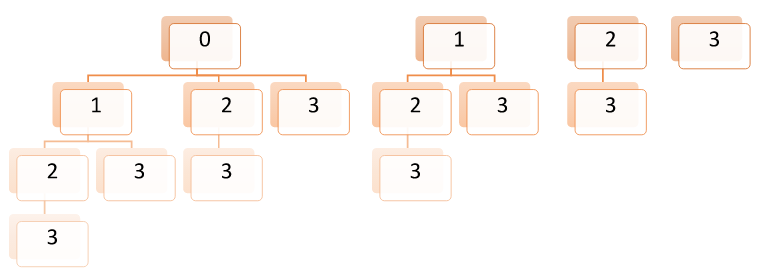
\includegraphics[width=0.8\textwidth]{obr/stavy.png}
	\caption{Vizualizace stavového prostoru pro $|V(G)|-A=4$. Množina $B$ pro daný stav obsahuje ty vrcholy grafu, jejichž čísla
		se vyskytují na cestě z tohoto stavu směrem do kořene. (Samotný kořen, který odpovídá prázdné množině, není zobrazen.)}
	\label{imgStavy}
\end{figure}
\subsection{Vlastnosti a časová složitost algoritmu}
\paragraph{Klasifikace úlohy}\mbox{}\newline
Z hlediska klasifikace úloh na procházení stavového prostoru je úloha nalezení minimálního
Steinerova stromu úlohou s omezenou velikostí stavového prostoru, která optimalizuje velikost podgrafu (stromu) a obecně musí prohledat celý stavový prostor, jež může však může prořezávat. Vždy je známá těsná spodní mez velikosti řešení, která odpovídá velikosti počtu uzlů v terminální množině.

\paragraph{Odhad časové složitosti algoritmu}\mbox{}\newline
V našem řešení lze snadno nahlédnou velikost stavového stromu, tj. počet jeho uzlů.
Tato velikost je rovna číslu $2^{|V(G)|-|A|}$, což odpovídá počtu podmnožin množiny o 
$|V(G)|-|A|$ prvcích. Přímo to vyplývá z popisu průchodu stavovým prostorem a pomoci přiblížit to může obrázek \ref{imgStavy}.

Skutečný počet testovaných stavů může být nižší díky prořezávání. Přesto je možné snadno nalézt graf $G=(V,E)$ a terminální množinu $A$ tak, aby program skutečně musel projít úplně celý stavový prostor. Jedno takové zadání je na obrázku \ref{imgWorst} a obecně jde o případ, kdy je
$G$ strom a $A$ obsahuje právě všechny jeho listy.
\begin{figure}[ht]
	\centering
	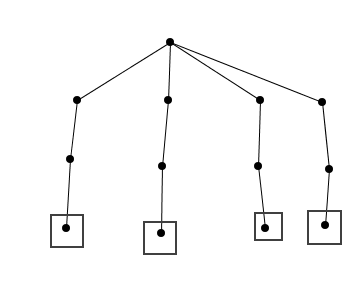
\includegraphics[width=0.4\textwidth]{obr/worst.png}
	\caption{Případ, kdy je vstupní graf strom a terminální množina obsahuje všechny jeho listy. Při tomto zadání se musí
		projít celý stavový prostor a vůbec se nemůže uplatnit prořezávání.}
	\label{imgWorst}
\end{figure}

Nejsložitější operací v cyklu systematického procházení stavů je testování souvislosti
grafu. Protože graf interně representujeme pomocí matice sousednosti, testujeme souvislost algoritmem přirozeným pro tuto representaci, který má časovou složitost $O(|E(G)|^2)$.

Jiné grafové representace by asi umožnili efektivnější testování souvislosti, ale my jsme zůstali u tohoto řešení, neboť to nijak nemění cíl a výsledek práce a zároveň je tato representace interně výhodná pro jednoduché testování souvislosti indukovaných podgrafů. Otestování
souvislosti indukovaného podgrafu o $k$ hranách trvá asymptoticky čas $O(k^2)$.

Složitost sekvenčního řešení v nejhorším případě je tedy asymptoticky rovna $O(2^{|V(G)|-|A|}\cdot |E(G)|^2)$.




\section{Popis paralelního algoritmu a jeho implementace v MPI}
Samotný princip procházení stavového stromu a jeho vlastnosti prezentované v předchozí sekci
platí i pro paralelní implementaci. Bylo pouze potřeba upravit některé použité datové struktury, aby
byly pro paralelní výpočet dobře použitelné (zejména zásobník).

Těžiště paralelního řešení leží v implementaci zprávově orientované komunikace mezi
jednotlivými procesy, možnosti dynamického rozdělování stavového prostoru do disjunktních podmnožin a jejich
přidělování procesům a zajištění správného ukončení výpočtu a zobrazení řešení.

Naše paralelní řešení popíšeme nejprve obecně, poté se podíváme podrobněji na některé důležité podrobnosti.
\subsection{Princip paralelní implementace}
Veškerou zprávově orientovanou komunikaci nám obstará knihovna MPI, která navíc obsahuje
taky další užitečně funkce, jako je zjištění celkového počtu procesů, na nichž úloha běží, nebo měření času výpočtu.

Naše implementace se na každý proces z globálního hlediska dívá jako na jednoduchý stavový automat, který
během výpočtu prochází různými stavy. Každý proces má svůj vlastní zásobník a k němu přidružený kontext,
pomocí kterých prochází a zpracovává určenou část stavového prostoru. Možné stavy procesů jsou následující.
\newline
\begin{center}
	\begin{tabular}{p{4cm}|p{8cm}}
		INIT & Označuje inicializační fázi, před samotným vstupem do cyklu, v němž se prochází stavový prostor.\\
		\hline
		WORKING & Proces má neprázdný zásobník, rozvíjí a testuje stavy stavového prostoru.\\
		\hline
		IDLE & Proces má prázdný zásobník. Nemá práci a je mu dovoleno žádat o přidělení práce nové.\\
		\hline
		IDLE\textunderscore EXPECTING & Proces nemá práci, ale požádal nějaký jiný proces o přidělení nové práce, a nyní
		očekává odpověď. Žádat znovu smí teprve až odpověď obdrží.\\
		\hline
		DONE & Proces je informován o tom, že celý stavový prostor už byl prozkoumán, a může opustit výpočetní cyklus.\\
	\end{tabular}
	\newline
\end{center}


Na začátku programu si každý proces sám přečte vstupní textový soubor se vstupními daty úlohy
a podle něj si vytvoří příslušné datové struktury. Poté proces číslo $0$, provede
iniciální rozdělení práce a to tak, že dostatečně rozvine stavový prostor a jeho kusy pošle ostatním procesům,
kteří si podle toho aktualizují svůj zásobník a kontext.

Procesy pak vstoupí do hlavního výpočetního cyklu, kde, podobně jako v sekvenčním případě, rozvíjí a ověřují
stavy v jim přidělené části stavového prostoru. Hlavní rozdíl spočívá ve dvou věcech.
\begin{itemize}
	\item Procesy pravidelně po jistém počtu průchodů cyklem (viz níže) kontrolují svou frontu zpráv. V případě,
	že nějaká zpráva dorazila, na to patřičně reagují.
	\item Pokud se procesu vyprázdní zásobník, nemůže cyklus jen tak opustit. Musí se pokusit hledat dárce, který
	mu přidělí práci novou. Opustit cyklus je možné až ve chvíli, kdy dorazí odpovídající zpráva, která explicitně
	oznamuje, že byl zpracován celý stavový prostor a výpočet může končit.
\end{itemize}

Procesy si mezi sebou vyměňují několik typů zpráv. Význam shrnuje následující tabulka.
\newline

\begin{centering}
	\begin{tabular}{p{4.5cm}|p{7.5cm}}
		MSG\textunderscore WORK\textunderscore REQUEST & Žádost příjemce o přidělení práce. \\
		\hline
		MSG\textunderscore WORK\textunderscore SENT & Zpráva obsahující
		zásobníkový rámec s jeho kontextem -- tj. novou práci pro příjemce. \\
		\hline
		MSG\textunderscore WORK\textunderscore EMPTY & Zpráva informující příjemce o tom, že odesilatel nemá práci, kterou by předal. \\
		\hline
		MSG\textunderscore TOKEN & Zpráva, v níž příjemce dostává token, který
		se používá pro indikaci ukončení výpočtu (viz dále). \\
		\hline
		MSG\textunderscore TERM & Informace příjemci o tom, že výpočet může skončit, neboť byl prohledán celý stavový prostor. \\
		\hline
		MSG\textunderscore ASK\textunderscore FOR\textunderscore BEST & Dotaz
		na délku nejlepšího horního odhadu velikosti řešení známého příjemci. \\
		\hline
		MSG\textunderscore RECEIVE\textunderscore BEST & Informace pro
		příjemce o délce nejlepšího horního odhadu velikosti řešení známé odesilateli. \\
	\end{tabular}
	\newline
\end{centering}


Když všechny procesy opustí výpočetní cyklus, je potřeba vypsat nalezené řešení.
Obecně nevíme, který proces toto řešení má. Může se dokonce stát, že budou mít dva procesy
různá řešení, protože, jak už bylo řečeno, nemusí být minimální Steinerův strom určen jednoznačně.
Připomeňme (viz část \ref{subPrincip}), že v tuto chvíli má řešení podobu souvislého indukovaného podgrafu, jehož kostra
je hledaný minimální Steinerův strom.

Provedeme tedy paralelní binární redukci (s využitím příslušné funkce MPI), jejímž výsledkem bude velikost
minimálního Steinerova stromu a nejmenší index procesu $i$ takový, že proces $i$ nalezl souvislý indukovaný podgraf této velikosti. Tento výsledek
paralelní binární redukce bude uložen v procesu $0$. Pokud $i=0$, pak sám tento proces sestrojí kostru tohoto grafu a vypíše řešení, jinak pošle zprávu procesu $i$,
který tyto kroky provede. Pak program může skončit.

\subsection{Klíčové části paralelní implementace}\label{subParkey}
\paragraph{Formát posílaných zpráv}
Posílání a příjem zpráv spolu s kontrolou fronty čekajících zpráv provádíme
pomocí odpovídajících funkcí knihovny MPI představených během výuky. Každý typ
zprávy je opatřen příslušným tagem (viz výše).

Formátem zprávy rozumíme formát jejího bufferu. Ten je až na jednu výjimku vždy jednoduchý
a obsahuje jedno nebo dvě celá čísla, jejichž povahu lze snadno vyvodit z výše
uvedené tabulky typů zpráv.

Zmíněnou výjimkou je zpráva, v níž dárce posílá žadateli část svého stavového prostoru.
Délka bufferu této zprávy je variabilní a obsahuje zásobníkový rámec, representující
vrchol stavového podprostoru, který začne příjemce zpracovávat, a dále kontext tohoto rámce.
V terminologii podsekce \ref{subPrincip} jde o posloupnost vrcholů grafu, které se pro tento rámec nachází
v podmnožině $B\subseteq V(G)$, která jednoznačně odpovídá právě jednomu indukovanému podgrafu v $G$,
jehož souvislost se bude testovat.

\paragraph{Taktika hledání dárce}\mbox{}\newline
Použili jsme taktiku lokálních cyklických žádostí. V inicializační fázi
si každý proces inicializuje svůj soukromý čítač pomocí pseudonáhodného
generátoru. Kdykoli pak proces chce žádat o práci, požádá o ni proces s číslem
rovným hodnotě svého čítače. Čítač pak inkrementuje o jedničku (modulo počet procesů),
přičemž se hlídá, aby proces nikdy nežádal o práci sebe sama.

\paragraph{Sdílení dílčích výsledků}
Jako výhodné se jeví sdílet informaci o horním odhadu velikosti hledaného minimálního Steinerova stromu, což umožňuje prořezávat části stavového prostoru. Používáme dvojí sdílení této
informace.
\begin{enumerate}
	\item \emph{Taktika piggybacking	}. Protože sdílenou informaci lze uložit do jediného celého čísla, posíláme tuto informaci spolu s každou jinou zprávou, kterou si procesy vymění. Stačí pouze zvětšit buffer posílaných zpráv o jedničku.
	\item \emph{Taktika distributora}. Ukázalo se, že předchozí taktika sama o sobě nemusí být dostačující. Proto jsme zvolili ještě přístup, kdy se vyhradí jeden z procesů -- tzv. distributor --  a ostatní mu pravidelně po určitém počtu $c$ iterací výpočetního cyklu posílají jim známý horní odhad velikosti řešení a na oplátku žádají jemu známý horní odhad. Hodnotu $c$ jsme volili experimentálně a řádově je větší, než je počet iterací, po kterém
	si procesy kontrolují své fronty zpráv. Konkrétně je $c\approx 2^{15}$.
\end{enumerate}
Zůstaňme ještě chvíli u taktiky distributora. Jak rychle se dostane nějaký dobrý odhad,
který nalezne jistý proces, ostatním procesům? Hrubou představu o tom
si lze učinit následující úvahou

	Označme $k$ celkový počet procesů řešících úlohu a nechť $P$ značí proces, který je distributorem horních
	odhadů velikosti řešení. Označme dále $c$ počet iterací výpočetního cyklu, po kterém ostatní
	procesy posílají distributorovi požadavek, a iterace výpočetního cyklu
	procesu $P$ rozdělme na fáze $F_i=\{0+ci, 1+ci, \dots, (c-1)+ci\},i\geq 0$.
	Pak platí.
\begin{tvrz}
	Pokud předpokládáme, že během každé fáze $F_i$ pošlou všechny ostatní procesy distributorovi po jednom požadavku a distributor stihne
	každému žadateli odpovědět a že pořadí zpráv v obou směrech je náhodné, pak
	daný proces $Q\neq P$ získá nejlepší odhad známý distributorovi během fáze $F_j$ nejpozději na konci fáze $F_{j+1}$ a
	s pravděpodobností přibližně aspoň
	$$\frac{1}{k}+\frac{k-1}{k}\cdot\frac{\frac{(k-1)!}{2}}{(k-1)!}=\frac{1}{k}+\frac{k-1}{k}\cdot\frac{1}{2}
	=\frac{k+1}{2k}>\frac{1}{2}$$
	jej získá již v samotné fázi $F_j$.
\end{tvrz}
\begin{proof}
	To, že každý žadatel obdrží zmíněný odhad nejpozději na konci následující fáze, plyne ihned z předpokladů, protože ve chvíli,
	kdy se bude proces dotazovat distributora v následující fázi, získá v nejhorším případě nejlepší odhad známý
	distributorovi v minulé fázi.
	
	Pravděpodobnost, že odhad obdrží ve stejné fázi lze odhadnout následující úvahou.
	Podle předpokladu je pořadí, v němž dorazí žádosti distributorovi, náhodné. Každé jedno takové pořadí
	lze jednoznačně representovat nějakou permutací množiny $M=\{0,1,\dots, k-2\}$. Tato čísla
	lze vzájemně jednoznačně namapovat na procesy-žadatele.
	
	Označme $R$ vlastníka nejlepšího odhadu v dané fázi. Pokud $P=R$, pak každý žadatel dostane řešení ještě
	v aktuální fázi. V opačném případě plyne z předchozího,
	že proces $Q\neq P$ se právě v polovině počtu možných pořadí bude nacházet za procesem $R$.
	Tedy v polovině případů mu $P$ odpoví ve chvíli, kdy už obdržel zprávu od $R$.
	
	Pro účely dolního odhadu předpokládejme, že v dané fázi zná nejlepší odhad pouze jediný proces, a že
	je náhodné, který proces to je. Odtud již plyne vztah uvedený v tvrzení.
\end{proof}

\paragraph{Způsob dělení zásobníku}
V paralelní implementaci používáme jako zásobník datovou strukturu v podobě oboustranné fronty, která umožňuje v čase $O(1)$ přidávat i odebírat
rámce ze svého začátku i konce.

Procesor během výpočtu zpracovává stavy z jednoho konce zásobníku (vrcholu) směrem ke druhému (dno). Platí důležitá vlastnost. Předpokládáme-li
značení vrcholů z $V(G)-A$ souvisle čísly $0, 1, \dots, N - 1 = |V(G)| - |A|$ a
použijeme-li značení rámců ze sekce ..., pak označíme-li $P(i,j)$ celkový počet stavů nacházejících se v podstromu stavového prostoru
s kořenem $(i,j)$, platí
$$P(i,j)=\sum_{k=i+1}^{N-1}P(k,j)-1$$
Vyplývá to z popisu procházení stavového prostoru v sekci \ref{subPrincip} a vizuálně
to přibližuje obrázek \ref{imgStavy}.

Tohoto pozorování se využívá při rozdělování zásobníku. Pokud má proces neprázdný zásobník, nachází se na jeho dně vždy rámec $(i,j)$, takový, že rámec s menší hodnotou první složky
se už v procesu aktuálně přiděleném stavovém podprostoru nikde neobjeví -- je to tedy rámec, obsahující největší možný počet potomků.

Právě z tohoto rámce proces-dárce přiděluje práci a to následovně.
\begin{enumerate}
	\item Pokud rámec na dně obsahuje \uv{dostatečný počet} podstavů (viz dále), přidělí dárce žadateli
	jeho největšího potomka (spolu s patřičným kontextem) a sám si jej ze svého prostoru
	odstraní.
	\item V opačném případě, kdy rámec dna už nemá dostatečný počet podstavů, ale zároveň
	stavový podprostor procesu-dárce obsahuje dostatek ještě neověřených stavů, přenechá
	dárce žadateli celý rámec svého dna.
	\item Pokud stavový podprostor dárce neobsahuje dostatek ještě neověřených stavů,
	je žadatel odmítnut.
\end{enumerate}
Vizuálně to demonstruje obrázek \ref{imgSplit}.
Jaké hodnotě odpovídá \uv{dostatečný počet} podstavů? Je to hodnota určená
na základě řezné výšky, což je koncept představený na přednášce. Konkrétně:
stavy, které obsahují méně než $h=15$ podúrovní (a tedy méně než $2^{15}$ podstavů), již nerozdělujeme.
\begin{figure}[ht]
	\centering
	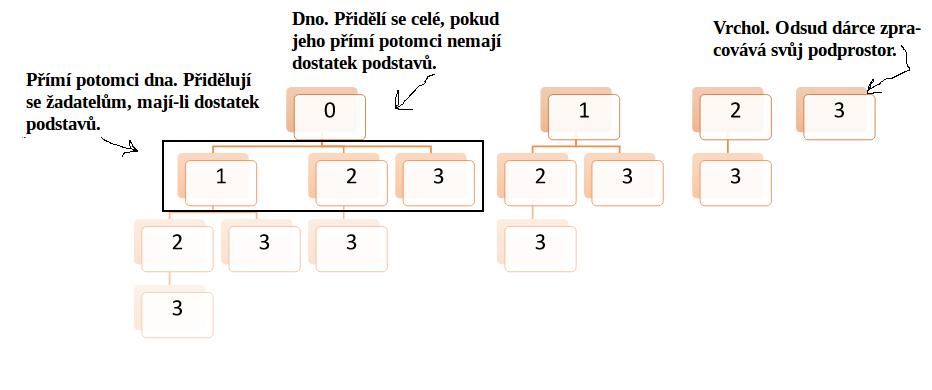
\includegraphics[width=1.0\textwidth]{obr/deleni.png}
	\caption{Zásobník a princip jeho dělení. Dárce zpracovává stavy směrem od vrcholu, kde
		jsou stavy s menším počtem potomků, a rozdává naopak potomky dna a nebo dno samotné.}
	\label{imgSplit}
\end{figure}
\paragraph{Způsob ukončení výpočtu}
Detekci ukončení výpočtu provádíme pomocí Dijkstrova algoritmu
pro paralelní výpočet s dynamickým vyvažováním zátěže. Implementujeme ho
přesně tak, jak byl prezentován během výuky. Viz např \cite[str. 490-491]{pars}.
\paragraph{Shrnutí důležitých výpočetních konstant}\mbox{}\newline
V této sekci bylo zmíněno v odpovídajících kontextech několik konstant,
které ovlivňují škálování algoritmu. Byly stanoveny experimentálně a částečně
podle doporučení z výuky. Jejich hodnoty je možné dle potřeby snadno změnit, neboť
jsou v programu definovány jako symbolické konstanty. Shrnutí obsahuje tabulka \ref{tabKonst}.
\begin{table}[ht]
\centering
\begin{tabular}{p{2.9cm}|r|p{7.6cm}}
	Konstanta [typ] & Hodnota & Popis\\
	\hline\hline
	m [celé číslo] & 200 & Počet cyklů výpočetního cyklu, po kterém procesy kontrolují své fronty zpráv.\\
	\hline
	c [celé číslo] & 32000 & Počet cyklů výpočetního cyklu, po kterém si procesy vyměňují s distributorem
	aktuálně známé odhady řešení.\\
	\hline
	h [celé číslo] & 15 & Řezná výška. Stavy s hloubkou menší než $h$ se už nerozdělují.\\
\end{tabular}
\caption{Shrnutí klíčových výpočetních konstant paralelní implementace. Jsou definovány jako
	symbolické konstanty a lze je snadno měnit a tím experimentovat s různými hodnotami.}\label{tabKonst}
\end{table}	

\section{Naměřené výsledky a vyhodnocení}
\paragraph{Instance zvolené pro měření}\mbox{}\newline
Pro účely měření a vyhodnocování výsledků jsme zvolili následující trojici instancí.
\begin{enumerate}
	\item Graf $G_1$ o $32$ uzlech, který je strom, a terminální množina $A$ obsahuje právě všechny jeho listy (pro ilustraci viz obrázek \ref{imgWorst}).
	Minimální Steinerův strom pro $A$ je v tomto případě samotný graf $G_1$, takže
	algoritmus musí projít úplně celý stavový prostor a vůbec se neuplatní prořezávání.
	
	Tuto instanci jsme zvolili záměrně, neboť z principu zde nedochází k žádnému superlineárnímu zrychlení.
	\item Graf $G_2$ s $40$ uzly s průměrným stupněm uzlu $4$. Terminální množina má velikost $9$ a byla volena náhodně.
	\item Graf $G_3$ s $42$ uzly a s průměrným stupněm uzlu $5$. Terminální množina má velikost $14$ uzlů a byla volena náhodně.
\end{enumerate}
\subsection{Paralelní čas a paralelní zrychlení}
Naším cílem bylo změřit paralelní čas pro všechny tři instance v situacích, kdy
algoritmus běžel po řadě na $1,2,4,8,16$ a $24$ procesorech. U grafů $G_2, G_3$ jsme
čas měřili i pro další počty procesorů, vzhledem k charakteru získaných výsledků. Tabulka \ref{tabTime} ukazuje
naměřené hodnoty paralelních časů. V příloze jsou pak zobrazeny grafy paralelních časů a zrychlení.

\begin{table}[ht]
	\centering
	\begin{tabular}{r|r|r|r}
		\#CPU & Čas pro $G_1$ [s]& Čas pro $G_2$ [s]& Čas pro $G_3 [s]$\\
		\hline\hline
		1 & $243$ & $247,9$ & $793$\\
		\hline
		2 & $124,8$ & $248,8$ & $172,8$\\
		\hline
		4 & $62,7$ & $248,7$ & $173,6$\\
		\hline
		5 & - & $248,4$ & $7,206$\\
		\hline
		6 & - & $249,1$ & $7,203$\\
		\hline
		7 & - & $14,4$ & $7,361$\\
		\hline
		8 & $31,17$ & $0,0159$ & $7,185$\\
		\hline
		12 & - & - & $7,229$\\
		\hline
		16 & $19,84$ & $0,081$ & $8,98$\\
		\hline
		24 & $17,52$ & $0,2868$ & $0,4711$\\
	
	\end{tabular}
	\caption{Naměřené paralelní časy pro zvolené instance problému. Prázdné políčko znamená,
		že pro odpovídající instanci a počet procesorů nebyl čas změřen.}
	\label{tabTime}
\end{table}
\subsection{Rozbor naměřených hodnot}
Rozebereme zvlášť výsledky pro instanci $G_1$ a pro dvojici instancí. $G_2, G_3$.
\paragraph{Rozbor instance $G_1$}\mbox{}\newline
Jak bylo uvedeno výše, je nutné v případě instance $G_1$ vždy projít celý stavový prostor -- vůbec se
neuplatní prořezávání stavového prostoru. Z principu zde tedy nemůže dojít k superlineárnímu zrychlení a v ideálním
případě očekáváme zrychlení lineární.

Jak plyne z tabulky \ref{tabTime}, do $8$ procesorů se to tak skutečně jeví, naměřený čas je vždy poloviční oproti času
při polovičním počtu procesorů. Při běhu na $16$ a $24$ procesorech to však vypadá, že zrychlení začíná mít sublineární charakter.
Čím to může být způsobeno?

Abychom si učinili představu, provedli jsme pro instanci $G_1$ speciální měření. Pro počty procesorů po řadě $1,2,4,8$ a $16$ jsme změřili,
kolik z celkového počtu cyklů výpočetního cyklu tráví jednotlivé procesory v aktivním stavu, tj. ve stavu, kdy mají neprázdný zásobník
a aktivně rozvíjejí a testují stavový prostor. Tabulka \ref{tabAnal} shrnuje naměřené hodnoty.

\begin{table}[ht]
	\centering
	\begin{tabular}{r|r|r}
		\#CPU & Čas [s]& Průměrné $\%$ aktivních cyklů na procesor\\
		\hline\hline
		1 & $243$ & $100$\\
		\hline
		2 & $124,8$ & $99,38$\\
		\hline
		4 & $62,7$ & $96,25$\\
		\hline
		
		8 & $31,17$ & $89,16$\\
		\hline
	
		16 & $19,84$ & $79,38$\\	
	\end{tabular}
	\caption{Průměrné procento aktivních cyklů na procesor během řešení instance $G_1$ pro různé počty procesorů.}
	\label{tabAnal}
\end{table}
Položili jsme si otázku, čím může být způsobem pokles procenta aktivních cyklů s rostoucím počtem procesorů.
Usuzovali jsme na možnou dvojí příčinu.
\begin{enumerate}
	\item Doba mezi odesláním žádosti o práci a vyzvednutím odpovědi z fronty zpráv  může být dlouhá, tzn. výpočet je nezanedbatelně zpomalen komunikační
	režií.
	\item Příliš mnoho žádostí o práci může být odmítnuto.
\end{enumerate}
Abychom blíže zjistili, co se vlastně děje. Provedli jsme pro instanci $G_1$ ještě jedno měření. Tentokrát jsme
měřili na $16$ a $24$ procesorech a zjišťovali jsme počet úspěšných žádostí o práci, počet neúspěšných žádostí o práci
a dále počty cyklů hlavního výpočetního cyklu, které v průměru uplynou mezi odesláním žádosti a vyzvednutím odpovědi s odmítnutím
z fronty zpráv (tj. žádostí,
jejichž výsledkem není pro příjemce nová práce.). Výsledek ukazuje tabulka \ref{tabDeep}.
\begin{table}[ht]
	\centering
	\begin{tabular}{r|r|r|r}
		\#CPU & \# úsp. žád. & \# neúsp. žád. & poměr úsp. / neúsp.\\
		\hline\hline
		$16$ & 391 & 1370 & $0,285$\\
		\hline
		$24$ & 568 & 2056 & $0,276$\\
		
	\end{tabular}
	\caption{Průměrné celkové počty úspěšných a neúspěšných žádosti o přidělení práce všech procesorů při řešení instance
		$G_1$ pro $16$ a $24$ procesorů. Doba, mezi odesláním žádosti a vyzvednutí odpovědi s odmítnutím trvá
		procesoru v průměru asi $w=20202$ cyklů v hlavním výpočetním cyklu.}
	\label{tabDeep}
\end{table}

Vidíme, že problém je nejspíše relativně velké procento odmítnutých žádostí o práci. Tento závěr poukazuje na
možnosti vylepšení taktiky hledání dárce a taktiky rozdělení zásobníku.
\paragraph{Rozbor instancí $G_2$ a $G_3$}\mbox{}\newline
Zbylé dvě instance ukazují typičtější chování naší implementace v případě, že je na vstupu
zadán nějaký pseudonáhodně vygenerovaný graf.

Typicky se v takovém případě stane, že vstup má tak \uv{šťastnou} podobu, že při sekvenčním řešení procesor
rychle narazí na nějaký dobrý horní odhad velikosti řešení, a je tudíž schopen prořezat velkou část stavového prostoru.

Necháme-li pak tutéž instanci řešit o několik procesorů více, není tím tato výhoda překonána. Podoba vstupu umožňuje
relativně brzy proříznout tak velkou část stavového prostoru, že se na jeho zbytku pozitivně vůbec neprojeví fakt, že úlohu řeší
větší počet procesorů. Přesně tohle ukazují naměřené hodnoty pro instanci $G_2$ pro $2$ až $6$ procesorů.

Druhým typickým jevem pak je superlineární zrychlení, které \uv{náhle} nastane při jistém počtu procesorů. Vidět je to
u obou instancí $G_2, G_3$. To je způsobeno tím, že do jistého počtu $n$ řešících procesorů zůstává nějaký
dobrý horní odhad velikosti řešení ukryt hluboko ve stavovém prostoru jistého procesoru a trvá dlouho, než na něj tento procesor narazí a nebo
daruje odpovídající podprostor nějakému žadateli.

Jakmile však řeší úlohu o jeden procesor víc, dojde k tomu, že nyní již existuje dostatečný počet žadatelů na to, aby
byl podprostor obsahující tento odhad relativně rychle předán nějakému žadateli, který tento odhad nalezne, následně jeho velikost
sdílí s ostatními a opět dojde k relativně velkému prořezání, které dramaticky urychlí výpočet.

Instance $G_2, G_3$ demonstrují, že se tyto jevy mohou projevit i opakovaně pro větší počty procesorů. Výsledkem je pak
typicky \uv{schodovitý} graf paralelního času.
\subsection{Dynamické vyvažování zátěže a granularita implementace}
\paragraph{Hledání dárce a dělení zásobníku}\mbox{}\newline
Dynamické vyvažování zátěže přímo souvisí s taktikou hledání dárce a dělením zásobníku. Ty jsou
popsány v části \ref{subParkey}.

Naše implementace dynamického vyvažování zátěže má své výhody a nevýhody. Samotná operace rozdělení
zásobníku trvá dárci vždy čas $O(1)$, dárce tedy není při dělení nijak zbytečně časově zatížen, což je výhoda.
Celková časová složitost komunikace mezi žadatelem a dárcem je tak v podstatě dána čistě časem potřebným k přenosu
zpráv s žádostí a odpovědí.

Na druhou stranu je tato efektivnost vykoupena tím, že rozdělení zátěže není plně rovnoměrné. Pokud požádají
dva procesy nějakého stejného dárce o práci, není oběma přidělena stejně velká část stavového prostoru, viz část \ref{subParkey}.
Naše implementace dělení je založena na tom, že dárce se snaží žadatele obdarovat relativně štědře, ovšem tak, aby ho to nestálo
zbytečné výpočty.

Při rozboru měřené instance $G_1$ jsme viděli, při větším počtu procesorů řešících úlohu, není kombinace naší
implementace dělení zásobníku a taktiky lokálních cyklických žádostí úplně ideální, neboť způsobuje, že nezanedbatelně
velké procento žádostí o přidělení nové práce skončí neúspěchem.

\paragraph{Meze pro rozklad výpočtu}\mbox{}\newline
Empiricky jsme stanovili, že nemá význam posílat procesům žádajícím o práci stavové podprostory
obsahující méně než $2^{15}$ stavů.

Pro všechna měření v tabulce \ref{tabTime} jsme pro zajímavost také změřili, kolik průměrně cyklů v hlavním
výpočetním cyklu stráví proces mezi odesláním žádosti o práci a vyzvednutím přímo následující odpovědi ze své fronty zpráv za předpokladu,
že tato odpověď je kladná, tj. obsahuje rozdělený zásobník. Průměrně je tento počet $f\approx 42000$. Na tom jsme založili volbu řezné výšky. 

\section{Závěr}
Sestavili jsme sekvenční algoritmus pro řešení problému nalezení minimálního Steinerova stromu
pomocí systematického prohledávání stavového prostoru.

Následně jsme řešení paralelizovali za pomoci knihovny MPI, která nám umožnila
zajistit zprávově orientovanou komunikaci mezi procesy, implementací jednoduchého
stavového automatu, který sleduje činnost každého procesu účastnícího se výpočtu, a 
realizací možnosti dynamicky vyvažovat výpočetní zátěž.

Na třech ukázkových instancí jsme naměřili paralelní časy a diskutovali jsme nad výsledky.
Co se týká návrhu na zlepšení, stálo by za to zamyslet se nad lepší taktikou dělení zásobníku
a hledáním dárce, které by dohromady zvýšily procento aktivních cyklů v hlavním výpočetním cyklu procesů.
\paragraph{Osobní poznatky a zkušenosti}\mbox{}
\paragraph{Libor Vytlačil:} Seznámil jsem se s mně doposud neznámou knihovnou MPI a získal
jsem základní zkušenost a poznatky při implementaci paralelní aplikace pomocí této knihovny.

\paragraph{Vladimír Mlázovský:} Oživil jsem si programování v C++ a zamyslel jsem se hlouběji nad paralelizací problému. Nenapadlo
by mě, že je až takový rozdíl mezi programováním vícevláknové aplikace a aplikace pro paralelní stroj.
\addcontentsline{toc}{section}{Reference}
\begin{thebibliography}{9}
	\bibitem{pars}
	GRAMA, Ananth. \emph{Introduction to parallel computing}. 2nd ed. Harlow: Addison-Wesley, 2003, xx, 636 s. ISBN 0201648652.
	\bibitem{npc}
	SANTUARI, Alessandro. \emph{Steiner Tree NP-completeness Proof} [online]. 2003 [cit. 2015-12-12]. Dostupné z: \url{http://profs.sci.univr.it/~rrizzi/classes/Complexity/provette/Santuari/steiner.pdf}	
\end{thebibliography}
\section*{Přílohy}
\addcontentsline{toc}{section}{Přílohy}
Zde jsou zobrazeny grafy naměřených hodnot.
\begin{figure}[ht]
	\centering
	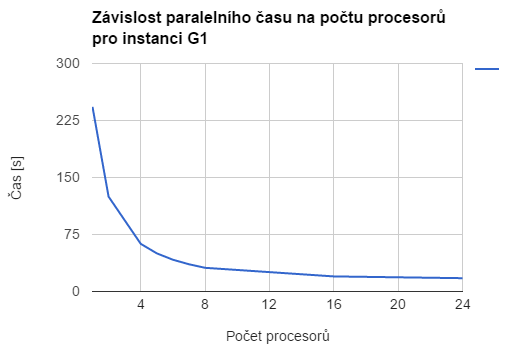
\includegraphics[width=0.90\textwidth]{obr/time1.png}
	\caption{Paralelní čas pro instanci $G_1$.}
	\label{imgTime1}
\end{figure}
\begin{figure}[ht]
	\centering
	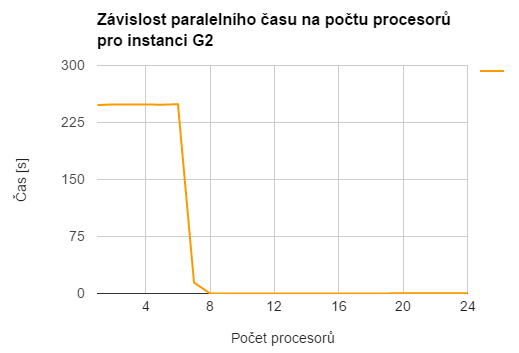
\includegraphics[width=0.90\textwidth]{obr/time2.png}
	\caption{Paralelní čas pro instanci $G_2$.}
	\label{imgTime2}
\end{figure}
\begin{figure}[ht]
	\centering
	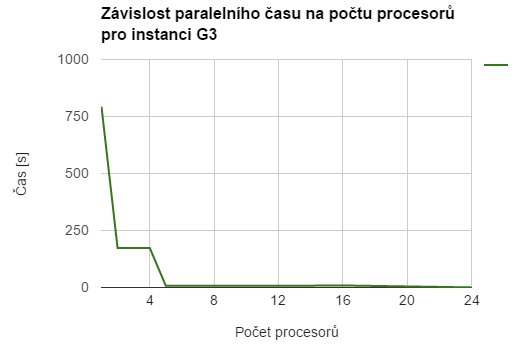
\includegraphics[width=0.90\textwidth]{obr/time3.png}
	\caption{Paralelní čas pro instanci $G_3$.}
	\label{imgTime3}
\end{figure}
\begin{figure}[ht]
	\centering
	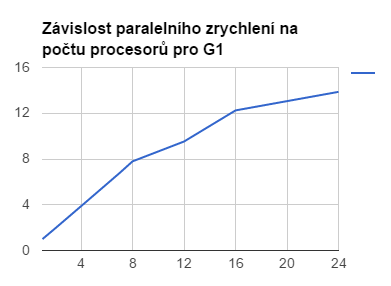
\includegraphics[width=0.75\textwidth]{obr/acc1.png}
	\caption{Paralelní zrychlení pro instanci $G_1$.}
	\label{imgAcc1}
\end{figure}
\begin{figure}[ht]
	\centering
	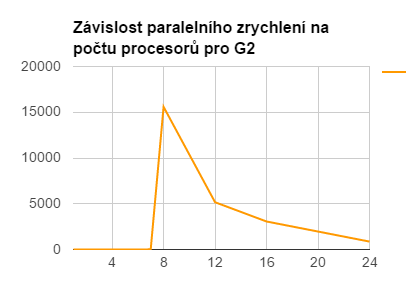
\includegraphics[width=0.75\textwidth]{obr/acc2.png}
	\caption{Paralelní zrychlení pro instanci $G_2$.}
	\label{imgAcc2}
\end{figure}
\begin{figure}[ht]
	\centering
	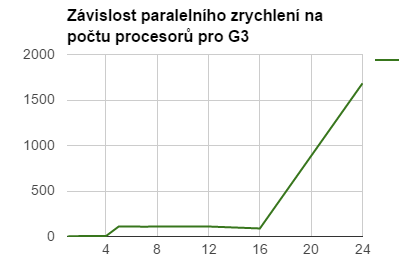
\includegraphics[width=0.75\textwidth]{obr/acc3.png}
	\caption{Paralelní zrychlení pro instanci $G_3$.}
	\label{imgAcc3}
\end{figure}
\end{document}